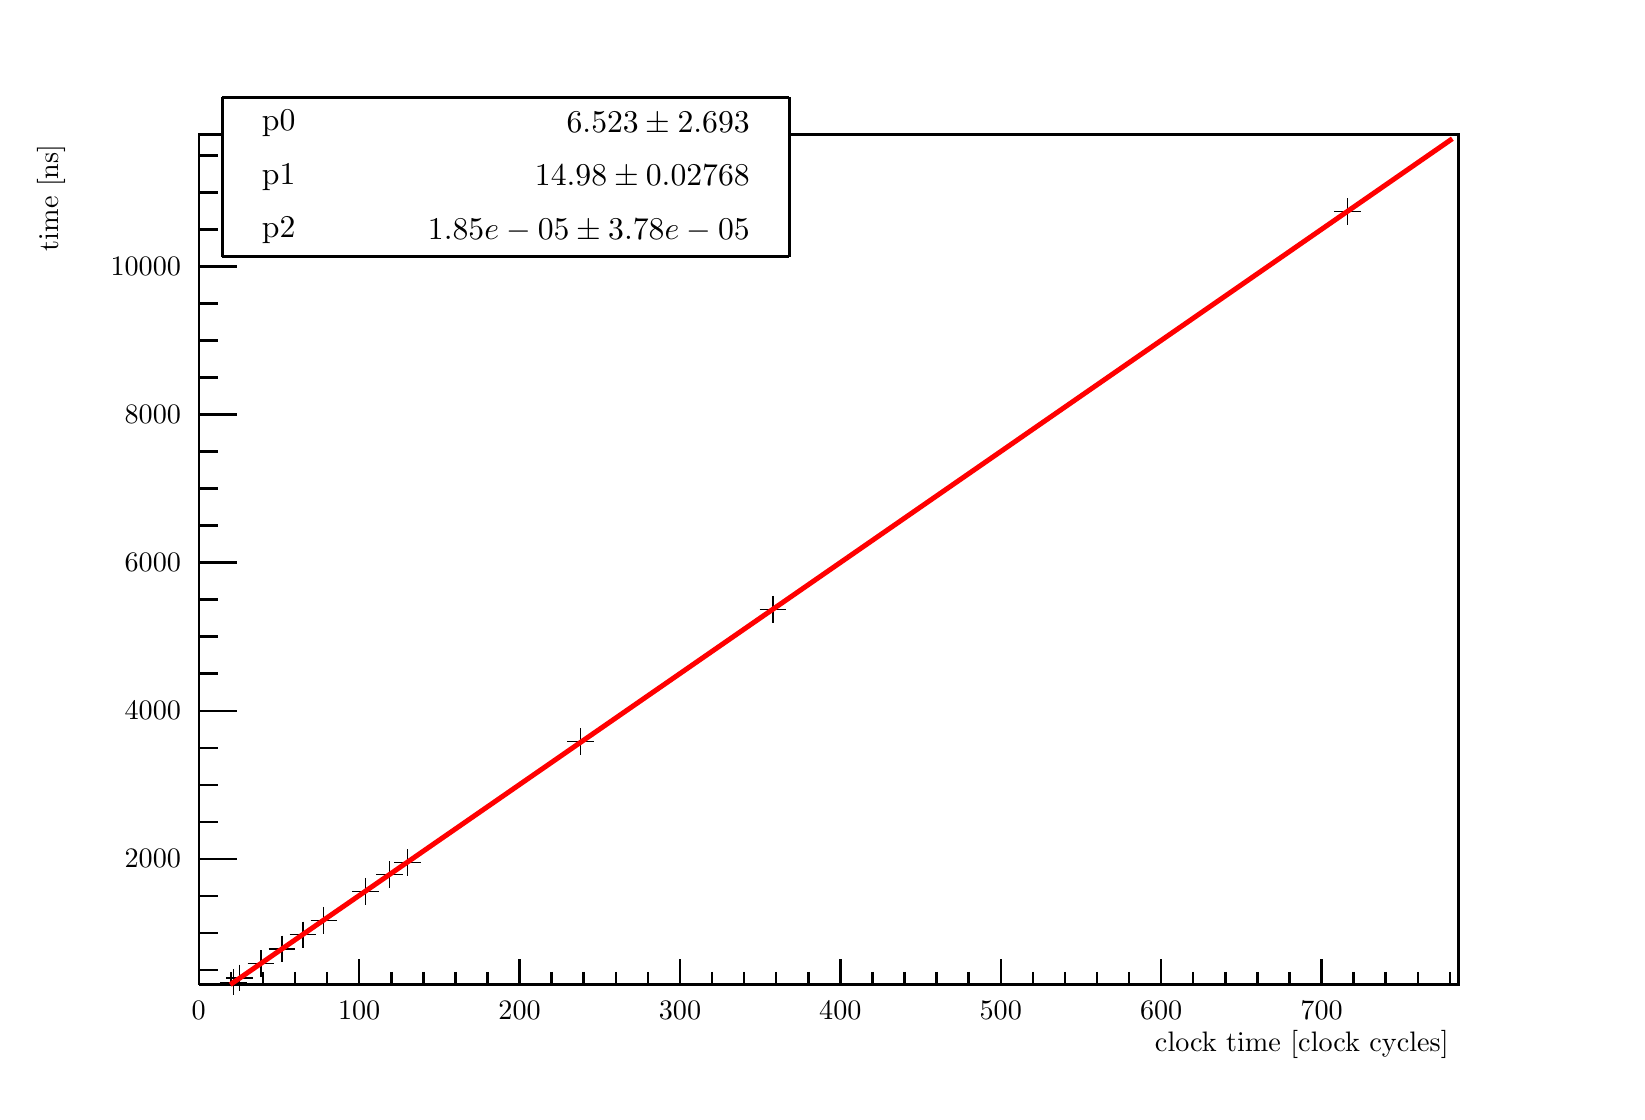
\begin{tikzpicture}
\pgfdeclareplotmark{cross} {
\pgfpathmoveto{\pgfpoint{-0.3\pgfplotmarksize}{\pgfplotmarksize}}
\pgfpathlineto{\pgfpoint{+0.3\pgfplotmarksize}{\pgfplotmarksize}}
\pgfpathlineto{\pgfpoint{+0.3\pgfplotmarksize}{0.3\pgfplotmarksize}}
\pgfpathlineto{\pgfpoint{+1\pgfplotmarksize}{0.3\pgfplotmarksize}}
\pgfpathlineto{\pgfpoint{+1\pgfplotmarksize}{-0.3\pgfplotmarksize}}
\pgfpathlineto{\pgfpoint{+0.3\pgfplotmarksize}{-0.3\pgfplotmarksize}}
\pgfpathlineto{\pgfpoint{+0.3\pgfplotmarksize}{-1.\pgfplotmarksize}}
\pgfpathlineto{\pgfpoint{-0.3\pgfplotmarksize}{-1.\pgfplotmarksize}}
\pgfpathlineto{\pgfpoint{-0.3\pgfplotmarksize}{-0.3\pgfplotmarksize}}
\pgfpathlineto{\pgfpoint{-1.\pgfplotmarksize}{-0.3\pgfplotmarksize}}
\pgfpathlineto{\pgfpoint{-1.\pgfplotmarksize}{0.3\pgfplotmarksize}}
\pgfpathlineto{\pgfpoint{-0.3\pgfplotmarksize}{0.3\pgfplotmarksize}}
\pgfpathclose
\pgfusepathqstroke
}
\pgfdeclareplotmark{cross*} {
\pgfpathmoveto{\pgfpoint{-0.3\pgfplotmarksize}{\pgfplotmarksize}}
\pgfpathlineto{\pgfpoint{+0.3\pgfplotmarksize}{\pgfplotmarksize}}
\pgfpathlineto{\pgfpoint{+0.3\pgfplotmarksize}{0.3\pgfplotmarksize}}
\pgfpathlineto{\pgfpoint{+1\pgfplotmarksize}{0.3\pgfplotmarksize}}
\pgfpathlineto{\pgfpoint{+1\pgfplotmarksize}{-0.3\pgfplotmarksize}}
\pgfpathlineto{\pgfpoint{+0.3\pgfplotmarksize}{-0.3\pgfplotmarksize}}
\pgfpathlineto{\pgfpoint{+0.3\pgfplotmarksize}{-1.\pgfplotmarksize}}
\pgfpathlineto{\pgfpoint{-0.3\pgfplotmarksize}{-1.\pgfplotmarksize}}
\pgfpathlineto{\pgfpoint{-0.3\pgfplotmarksize}{-0.3\pgfplotmarksize}}
\pgfpathlineto{\pgfpoint{-1.\pgfplotmarksize}{-0.3\pgfplotmarksize}}
\pgfpathlineto{\pgfpoint{-1.\pgfplotmarksize}{0.3\pgfplotmarksize}}
\pgfpathlineto{\pgfpoint{-0.3\pgfplotmarksize}{0.3\pgfplotmarksize}}
\pgfpathclose
\pgfusepathqfillstroke
}
\pgfdeclareplotmark{newstar} {
\pgfpathmoveto{\pgfqpoint{0pt}{\pgfplotmarksize}}
\pgfpathlineto{\pgfqpointpolar{44}{0.5\pgfplotmarksize}}
\pgfpathlineto{\pgfqpointpolar{18}{\pgfplotmarksize}}
\pgfpathlineto{\pgfqpointpolar{-20}{0.5\pgfplotmarksize}}
\pgfpathlineto{\pgfqpointpolar{-54}{\pgfplotmarksize}}
\pgfpathlineto{\pgfqpointpolar{-90}{0.5\pgfplotmarksize}}
\pgfpathlineto{\pgfqpointpolar{234}{\pgfplotmarksize}}
\pgfpathlineto{\pgfqpointpolar{198}{0.5\pgfplotmarksize}}
\pgfpathlineto{\pgfqpointpolar{162}{\pgfplotmarksize}}
\pgfpathlineto{\pgfqpointpolar{134}{0.5\pgfplotmarksize}}
\pgfpathclose
\pgfusepathqstroke
}
\pgfdeclareplotmark{newstar*} {
\pgfpathmoveto{\pgfqpoint{0pt}{\pgfplotmarksize}}
\pgfpathlineto{\pgfqpointpolar{44}{0.5\pgfplotmarksize}}
\pgfpathlineto{\pgfqpointpolar{18}{\pgfplotmarksize}}
\pgfpathlineto{\pgfqpointpolar{-20}{0.5\pgfplotmarksize}}
\pgfpathlineto{\pgfqpointpolar{-54}{\pgfplotmarksize}}
\pgfpathlineto{\pgfqpointpolar{-90}{0.5\pgfplotmarksize}}
\pgfpathlineto{\pgfqpointpolar{234}{\pgfplotmarksize}}
\pgfpathlineto{\pgfqpointpolar{198}{0.5\pgfplotmarksize}}
\pgfpathlineto{\pgfqpointpolar{162}{\pgfplotmarksize}}
\pgfpathlineto{\pgfqpointpolar{134}{0.5\pgfplotmarksize}}
\pgfpathclose
\pgfusepathqfillstroke
}
\definecolor{c}{rgb}{1,1,1};
\draw [color=c, fill=c] (0,0) rectangle (20,13.4957);
\draw [color=c, fill=c] (2,1.34957) rectangle (18,12.1461);
\definecolor{c}{rgb}{0,0,0};
\draw [c,line width=0.9] (2,1.34957) -- (2,12.1461) -- (18,12.1461) -- (18,1.34957) -- (2,1.34957);
\definecolor{c}{rgb}{1,1,1};
\draw [color=c, fill=c] (2,1.34957) rectangle (18,12.1461);
\definecolor{c}{rgb}{0,0,0};
\draw [c,line width=0.9] (2,1.34957) -- (2,12.1461) -- (18,12.1461) -- (18,1.34957) -- (2,1.34957);
\draw [c,line width=0.9] (2,1.34957) -- (18,1.34957);
\draw [c,line width=0.9] (2,1.67347) -- (2,1.34957);
\draw [c,line width=0.9] (2.40741,1.51152) -- (2.40741,1.34957);
\draw [c,line width=0.9] (2.81482,1.51152) -- (2.81482,1.34957);
\draw [c,line width=0.9] (3.22223,1.51152) -- (3.22223,1.34957);
\draw [c,line width=0.9] (3.62964,1.51152) -- (3.62964,1.34957);
\draw [c,line width=0.9] (4.03705,1.67347) -- (4.03705,1.34957);
\draw [c,line width=0.9] (4.44446,1.51152) -- (4.44446,1.34957);
\draw [c,line width=0.9] (4.85187,1.51152) -- (4.85187,1.34957);
\draw [c,line width=0.9] (5.25928,1.51152) -- (5.25928,1.34957);
\draw [c,line width=0.9] (5.66669,1.51152) -- (5.66669,1.34957);
\draw [c,line width=0.9] (6.0741,1.67347) -- (6.0741,1.34957);
\draw [c,line width=0.9] (6.48151,1.51152) -- (6.48151,1.34957);
\draw [c,line width=0.9] (6.88892,1.51152) -- (6.88892,1.34957);
\draw [c,line width=0.9] (7.29633,1.51152) -- (7.29633,1.34957);
\draw [c,line width=0.9] (7.70374,1.51152) -- (7.70374,1.34957);
\draw [c,line width=0.9] (8.11115,1.67347) -- (8.11115,1.34957);
\draw [c,line width=0.9] (8.51856,1.51152) -- (8.51856,1.34957);
\draw [c,line width=0.9] (8.92597,1.51152) -- (8.92597,1.34957);
\draw [c,line width=0.9] (9.33338,1.51152) -- (9.33338,1.34957);
\draw [c,line width=0.9] (9.74079,1.51152) -- (9.74079,1.34957);
\draw [c,line width=0.9] (10.1482,1.67347) -- (10.1482,1.34957);
\draw [c,line width=0.9] (10.5556,1.51152) -- (10.5556,1.34957);
\draw [c,line width=0.9] (10.963,1.51152) -- (10.963,1.34957);
\draw [c,line width=0.9] (11.3704,1.51152) -- (11.3704,1.34957);
\draw [c,line width=0.9] (11.7778,1.51152) -- (11.7778,1.34957);
\draw [c,line width=0.9] (12.1852,1.67347) -- (12.1852,1.34957);
\draw [c,line width=0.9] (12.5927,1.51152) -- (12.5927,1.34957);
\draw [c,line width=0.9] (13.0001,1.51152) -- (13.0001,1.34957);
\draw [c,line width=0.9] (13.4075,1.51152) -- (13.4075,1.34957);
\draw [c,line width=0.9] (13.8149,1.51152) -- (13.8149,1.34957);
\draw [c,line width=0.9] (14.2223,1.67347) -- (14.2223,1.34957);
\draw [c,line width=0.9] (14.6297,1.51152) -- (14.6297,1.34957);
\draw [c,line width=0.9] (15.0371,1.51152) -- (15.0371,1.34957);
\draw [c,line width=0.9] (15.4445,1.51152) -- (15.4445,1.34957);
\draw [c,line width=0.9] (15.8519,1.51152) -- (15.8519,1.34957);
\draw [c,line width=0.9] (16.2593,1.67347) -- (16.2593,1.34957);
\draw [c,line width=0.9] (16.2593,1.67347) -- (16.2593,1.34957);
\draw [c,line width=0.9] (16.6668,1.51152) -- (16.6668,1.34957);
\draw [c,line width=0.9] (17.0742,1.51152) -- (17.0742,1.34957);
\draw [c,line width=0.9] (17.4816,1.51152) -- (17.4816,1.34957);
\draw [c,line width=0.9] (17.889,1.51152) -- (17.889,1.34957);
\draw [anchor=base] (2,0.904212) node[scale=1.01821, color=c, rotate=0]{0};
\draw [anchor=base] (4.03705,0.904212) node[scale=1.01821, color=c, rotate=0]{100};
\draw [anchor=base] (6.0741,0.904212) node[scale=1.01821, color=c, rotate=0]{200};
\draw [anchor=base] (8.11115,0.904212) node[scale=1.01821, color=c, rotate=0]{300};
\draw [anchor=base] (10.1482,0.904212) node[scale=1.01821, color=c, rotate=0]{400};
\draw [anchor=base] (12.1852,0.904212) node[scale=1.01821, color=c, rotate=0]{500};
\draw [anchor=base] (14.2223,0.904212) node[scale=1.01821, color=c, rotate=0]{600};
\draw [anchor=base] (16.2593,0.904212) node[scale=1.01821, color=c, rotate=0]{700};
\draw [anchor= east] (18,0.593811) node[scale=1.01821, color=c, rotate=0]{clock time [clock cycles]};
\draw [c,line width=0.9] (2,1.34957) -- (2,12.1461);
\draw [c,line width=0.9] (2.48,2.94679) -- (2,2.94679);
\draw [c,line width=0.9] (2.24,3.41697) -- (2,3.41697);
\draw [c,line width=0.9] (2.24,3.88716) -- (2,3.88716);
\draw [c,line width=0.9] (2.24,4.35734) -- (2,4.35734);
\draw [c,line width=0.9] (2.48,4.82752) -- (2,4.82752);
\draw [c,line width=0.9] (2.24,5.29771) -- (2,5.29771);
\draw [c,line width=0.9] (2.24,5.76789) -- (2,5.76789);
\draw [c,line width=0.9] (2.24,6.23808) -- (2,6.23808);
\draw [c,line width=0.9] (2.48,6.70826) -- (2,6.70826);
\draw [c,line width=0.9] (2.24,7.17845) -- (2,7.17845);
\draw [c,line width=0.9] (2.24,7.64863) -- (2,7.64863);
\draw [c,line width=0.9] (2.24,8.11881) -- (2,8.11881);
\draw [c,line width=0.9] (2.48,8.589) -- (2,8.589);
\draw [c,line width=0.9] (2.24,9.05918) -- (2,9.05918);
\draw [c,line width=0.9] (2.24,9.52937) -- (2,9.52937);
\draw [c,line width=0.9] (2.24,9.99955) -- (2,9.99955);
\draw [c,line width=0.9] (2.48,10.4697) -- (2,10.4697);
\draw [c,line width=0.9] (2.48,2.94679) -- (2,2.94679);
\draw [c,line width=0.9] (2.24,2.4766) -- (2,2.4766);
\draw [c,line width=0.9] (2.24,2.00642) -- (2,2.00642);
\draw [c,line width=0.9] (2.24,1.53623) -- (2,1.53623);
\draw [c,line width=0.9] (2.48,10.4697) -- (2,10.4697);
\draw [c,line width=0.9] (2.24,10.9399) -- (2,10.9399);
\draw [c,line width=0.9] (2.24,11.4101) -- (2,11.4101);
\draw [c,line width=0.9] (2.24,11.8803) -- (2,11.8803);
\draw [anchor= east] (1.9,2.94679) node[scale=1.01821, color=c, rotate=0]{2000};
\draw [anchor= east] (1.9,4.82752) node[scale=1.01821, color=c, rotate=0]{4000};
\draw [anchor= east] (1.9,6.70826) node[scale=1.01821, color=c, rotate=0]{6000};
\draw [anchor= east] (1.9,8.589) node[scale=1.01821, color=c, rotate=0]{8000};
\draw [anchor= east] (1.9,10.4697) node[scale=1.01821, color=c, rotate=0]{10000};
\draw [anchor= east] (0.125215,12.1461) node[scale=1.01821, color=c, rotate=90]{time [ns]};
\draw [c,line width=0.9] (2.43797,1.38107) -- (2.51464,1.43373) -- (2.78973,1.61711) -- (3.05643,1.80142) -- (3.32321,1.98197) -- (3.5891,2.16722) -- (4.12028,2.53585) -- (4.42409,2.74931) -- (4.65112,2.90259) -- (6.84818,4.43351) --
 (9.29263,6.11677) -- (16.5853,11.1675);
\foreach \P in {(2.43797,1.38107), (2.51464,1.43373), (2.78973,1.61711), (3.05643,1.80142), (3.32321,1.98197), (3.5891,2.16722), (4.12028,2.53585), (4.42409,2.74931), (4.65112,2.90259), (6.84818,4.43351), (9.29263,6.11677),
 (16.5853,11.1675)}{\draw[mark options={color=c,fill=c},mark size=4.804805pt,mark=+] plot coordinates {\P};}
\definecolor{c}{rgb}{1,0,0};
\draw [c,line width=1.8] (2.4,1.34957) -- (2.56,1.45948) -- (2.72,1.57013) -- (2.88,1.6808) -- (3.04,1.79146) -- (3.2,1.90213) -- (3.36,2.01279) -- (3.52,2.12346) -- (3.68,2.23414) -- (3.84,2.34481) -- (4,2.45549) -- (4.16,2.56617) -- (4.32,2.67685)
 -- (4.48,2.78753) -- (4.64,2.89822) -- (4.8,3.0089) -- (4.96,3.11959) -- (5.12,3.23029) -- (5.28,3.34098) -- (5.44,3.45168) -- (5.6,3.56237) -- (5.76,3.67307) -- (5.92,3.78378) -- (6.08,3.89448) -- (6.24,4.00519) -- (6.4,4.1159) -- (6.56,4.22661) --
 (6.72,4.33732) -- (6.88,4.44804) -- (7.04,4.55875) -- (7.2,4.66947) -- (7.36,4.7802) -- (7.52,4.89092) -- (7.68,5.00165) -- (7.84,5.11237) -- (8,5.2231) -- (8.16,5.33384) -- (8.32,5.44457) -- (8.48,5.55531) -- (8.64,5.66605) -- (8.8,5.77679) --
 (8.96,5.88753) -- (9.12,5.99828) -- (9.28,6.10903) -- (9.44,6.21978) -- (9.6,6.33053) -- (9.76,6.44128) -- (9.92,6.55204) -- (10.08,6.6628) -- (10.24,6.77356);
\draw [c,line width=1.8] (10.24,6.77356) -- (10.4,6.88432) -- (10.56,6.99508) -- (10.72,7.10585) -- (10.88,7.21662) -- (11.04,7.32739) -- (11.2,7.43816) -- (11.36,7.54894) -- (11.52,7.65972) -- (11.68,7.7705) -- (11.84,7.88128) -- (12,7.99206) --
 (12.16,8.10285) -- (12.32,8.21364) -- (12.48,8.32443) -- (12.64,8.43522) -- (12.8,8.54602) -- (12.96,8.65681) -- (13.12,8.76761) -- (13.28,8.87841) -- (13.44,8.98922) -- (13.6,9.10002) -- (13.76,9.21083) -- (13.92,9.32164) -- (14.08,9.43245) --
 (14.24,9.54327) -- (14.4,9.65408) -- (14.56,9.7649) -- (14.72,9.87572) -- (14.88,9.98654) -- (15.04,10.0974) -- (15.2,10.2082) -- (15.36,10.319) -- (15.52,10.4299) -- (15.68,10.5407) -- (15.84,10.6515) -- (16,10.7624) -- (16.16,10.8732) --
 (16.32,10.984) -- (16.48,11.0949) -- (16.64,11.2057) -- (16.8,11.3166) -- (16.96,11.4274) -- (17.12,11.5383) -- (17.28,11.6491) -- (17.44,11.76) -- (17.6,11.8709) -- (17.76,11.9817) -- (17.92,12.0926);
\definecolor{c}{rgb}{1,1,1};
\draw [color=c, fill=c] (2.3,10.5941) rectangle (9.5,12.6185);
\definecolor{c}{rgb}{0,0,0};
\draw [c,line width=0.9] (2.3,10.5941) -- (9.5,10.5941);
\draw [c,line width=0.9] (9.5,10.5941) -- (9.5,12.6185);
\draw [c,line width=0.9] (9.5,12.6185) -- (2.3,12.6185);
\draw [c,line width=0.9] (2.3,12.6185) -- (2.3,10.5941);
\draw [anchor= west] (2.66,12.2811) node[scale=1.14549, color=c, rotate=0]{p0       };
\draw [anchor= east] (9.14,12.2811) node[scale=1.14549, color=c, rotate=0]{$ 6.523 \pm 2.693$};
\draw [anchor= west] (2.66,11.6063) node[scale=1.14549, color=c, rotate=0]{p1       };
\draw [anchor= east] (9.14,11.6063) node[scale=1.14549, color=c, rotate=0]{$ 14.98 \pm 0.02768$};
\draw [anchor= west] (2.66,10.9315) node[scale=1.14549, color=c, rotate=0]{p2       };
\draw [anchor= east] (9.14,10.9315) node[scale=1.14549, color=c, rotate=0]{$ 1.85e-05 \pm 3.78e-05$};
\definecolor{c}{rgb}{1,1,1};
\draw [color=c, fill=c] (2.3,10.5941) rectangle (9.5,12.6185);
\definecolor{c}{rgb}{0,0,0};
\draw [c,line width=0.9] (2.3,10.5941) -- (9.5,10.5941);
\draw [c,line width=0.9] (9.5,10.5941) -- (9.5,12.6185);
\draw [c,line width=0.9] (9.5,12.6185) -- (2.3,12.6185);
\draw [c,line width=0.9] (2.3,12.6185) -- (2.3,10.5941);
\draw [anchor= west] (2.66,12.2811) node[scale=1.14549, color=c, rotate=0]{p0       };
\draw [anchor= east] (9.14,12.2811) node[scale=1.14549, color=c, rotate=0]{$ 6.523 \pm 2.693$};
\draw [anchor= west] (2.66,11.6063) node[scale=1.14549, color=c, rotate=0]{p1       };
\draw [anchor= east] (9.14,11.6063) node[scale=1.14549, color=c, rotate=0]{$ 14.98 \pm 0.02768$};
\draw [anchor= west] (2.66,10.9315) node[scale=1.14549, color=c, rotate=0]{p2       };
\draw [anchor= east] (9.14,10.9315) node[scale=1.14549, color=c, rotate=0]{$ 1.85e-05 \pm 3.78e-05$};
\end{tikzpicture}
